\documentclass{article}
\usepackage{amsmath}
\usepackage{amssymb}
\usepackage{amsthm}
\usepackage{graphicx} % Required for inserting images
\usepackage[margin=1in]{geometry} % Adjusted margins for better readability
\usepackage{enumitem} % Improved formatting for lists
%\usepackage{xcolor} % Required for defining colors
\usepackage{mdframed} % Required for framing the NOTE sections
\usepackage[usenames,dvipsnames,svgnames,table]{xcolor}
\usepackage{mathtools}
\DeclarePairedDelimiter\ceil{\lceil}{\rceil}
\DeclarePairedDelimiter\floor{\lfloor}{\rfloor}
\usepackage{hyperref}
\hypersetup{
     colorlinks   = true,
     citecolor    = gray
}

\usepackage{tocloft}

\renewcommand{\cftsubsecfont}{\normalfont\hypersetup{linkcolor=purple}}
\renewcommand{\cftsubsecafterpnum}{\hypersetup{linkcolor=blue}}

% Define a color for the box
\definecolor{lightblue}{RGB}{173, 216, 230}

% Define a framed box for notes
\mdfdefinestyle{MyFrame}{%
    backgroundcolor=lightblue,
    roundcorner=5pt,
    frametitlerule=true,
    frametitlebackgroundcolor=white,
    frametitlerulecolor=lightblue,
    innertopmargin=\topskip,
}

\definecolor{lightorangered}{RGB}{255, 200, 173}

% Define a framed box for notes
\mdfdefinestyle{HW}{%
    backgroundcolor=lightorangered,
    roundcorner=5pt,
    frametitlerule=true,
    frametitlebackgroundcolor=white,
    frametitlerulecolor=lightblue,
    innertopmargin=\topskip,
}

% Define a color for the box
\definecolor{lightblue}{RGB}{173, 216, 230}

% Define a framed box for notes
\mdfdefinestyle{MyFrame}{%
    backgroundcolor=lightblue,
    roundcorner=5pt,
    frametitlerule=true,
    frametitlebackgroundcolor=white,
    frametitlerulecolor=lightblue,
    innertopmargin=\topskip,
}
% Define a framed box for notes
\mdfdefinestyle{MyFrame}{%
    backgroundcolor=lightblue,
    roundcorner=5pt,
    frametitlerule=true,
    frametitlebackgroundcolor=white,
    frametitlerulecolor=lightblue,
    innertopmargin=\topskip,
}
%permuatation and comb
\newcommand*{\permcomb}[4][0mu]{{{}^{#3}\mkern#1#2_{#4}}}
\newcommand*{\perm}[1][-3mu]{\permcomb[#1]{P}}
\newcommand*{\comb}[1][-1mu]{\permcomb[#1]{C}}
% Define a box for class session dates
\usepackage[most]{tcolorbox}

\NewTColorBox{classsessionbox}{O{}}{
    colback=white,
    colframe=lightblue,
    arc=0pt,
    outer arc=0pt,
    leftrule=0pt,
    rightrule=0pt,
    toprule=0pt,
    bottomrule=0pt,
    boxrule=0pt,
    right=0pt,
    top=5pt,
    bottom=5pt,
    width=3cm, % Set the width as needed
    title={\textbf{#1}},
    fontupper=\small, % Adjust the font size as needed
    halign=flush right, % Align to the right
}


\makeindex

% Define a theorem style
\theoremstyle{definition}
\newtheorem{theorem}{Theorem}


\title{Probability Class Notes}
\author{Shuvam Banerji Seal}
\date{January 2024}
\date{\today} % Adjusted to include the current date

\begin{document}

\maketitle
\tableofcontents

\section{Class Session 3: 3rd January 2024\\ Introduction to Probability}

\subsection{Axioms of Probability}
Sample Space ($\Omega$): The set of all outcomes of an experiment.
Space of events and the axioms of probability:
The space of events is a certain set of the power set of ($\Omega$).
\begin{enumerate}
    \item $\Omega \in \epsilon$
    \item If $A \in \epsilon$, then $A^c \in \epsilon$
    \item If $A_{i=1}^{\infty}$ are events, then $\bigcup_{i=1}^{\infty} A_i \in \epsilon$
    \item Consider P:$\epsilon \to [0, 1]$ such that $P(\Omega) = 1$,
    and if $A_{i=1}^{\infty}$ are pairwise disjoint (i.e., $A_i \cap A_j = \phi$ if $i \neq j$), then
    $P\left(\bigcup_{i=1}^{\infty} A_i\right) = \sum_{i=1}^{\infty} P(A_i)$
\end{enumerate}

\subsubsection{Example 1:}
Tossing a coin: $\Omega = \{H, T\}$,
$\epsilon = \{\phi, \{H\}, \{T\}, \{H, T\}\}$
\[ P(\phi) = 0, \quad P(H) = p, \quad P(T) = 1-p, \quad P(\Omega) = 1 \]

\subsubsection{Example 2:}
Rolling a die: $\Omega = \{1,2,3,4,5,6\}$

\subsubsection{Example 3:}
Guessing the first letter of the person's name: $\Omega = \{A, B, \dots, Z\}$

\subsubsection{Example 4:}
Guessing the number of stars in the Milky Way: $\Omega = \{1,2,3, \dots \}$

\subsubsection{Example 5:}
Guessing someone's palm temperature (in $\degree $F): $\Omega = [55,115]$

\subsubsection{Example 6 (Anubhav):}
[ A = \text{Someone has fever} ]
[ A = [c, 115] \text{ for some } c ]
\[ A^c = [55, c] \]

$\epsilon = \{\phi, A, A^c, \Omega\}$
\begin{mdframed}[style=MyFrame]
\textbf{NOTE:}
Vita-Li set where probability can't be defined due to the sample space being $\infty$.
% Reminder to color it later using tikz
\end{mdframed}
% Reminder to color it later using tikz

\subsection{Definitions:}
\subsubsection{Mutually Exclusive Events:}
$A, B \in \epsilon$ are called MEE if $A \cap B = \phi$.
    Then, $P(A \cup B) = P(A) + P(B)$.
\begin{proof}
     When $A \cap B \neq \phi$,
    \[ A = (A \cap B^c) \cup (A \cap B) \]
    \[ P(A) = P(A \cap B^c) + P(A \cap B) \]
    \[ A \cup B = B \cup (A \cap B^c) \]
    \[ P(A \cup B) = P(B) + P(A \cap B^c) \]
    \[ P(A \cap B^c) = P(A \cup B) - P(B) \]
    \[ P(A) = P(A \cup B) - P(B) + P(A \cap B) \]
    \[ P(A \cup B) = P(A) + P(B) - P(A \cap B) \]
\end{proof}
    
    \begin{mdframed}[style =MyFrame]
         \textbf{Notes:} By induction, this notion can be generalized for arbitrary $n \in \mathbb{N}$.
         
    \textbf{Notes\_2:} 
    \begin{equation}
        |A \cup B| = |A| + |B| - |A \cap B|
    \end{equation}
    \begin{equation}
        | A_1 \cup A_2 \cup \dots \cup A_n| = \sum_{i=1}^{n}|A_i| - \sum_{i,j}^{n}|A_i \cap B_j|
    \end{equation}
    \[ P\left( \bigcup_{i=1}^{n}A_i\right) = -(-1)^1\sum_{i{_1}=1}^{n}P(A_{i_1}) \]
    \[ \ldots-(-1)^n \sum_{1\leq i_{1}<i_{2}<i_{3}<\ldots <i_{n}\leq n}^{n}P(A_{i_1}\cap A_{i_2}\cap A_{i_3}\cap \ldots \cap A_{i_n}) \]

    \dots Principle of Exclusion and Inclusion
         
    \end{mdframed}
   

 \subsubsection{Exhaustive Set of events:} A set $S \subset \epsilon$ is an exhaustive set of events (or the events in $S$ to be exhaustive) if $\bigcup_{A \in S} A = \Omega$.

    Let $\Omega = \{W_n\}_{n=1}^{\infty}$ be a countable sample space such that $\epsilon = 2^{\Omega}$,
    where $W_n \in \epsilon$ for all $W_n \in \Omega$.

    Now, we have
    \[ 1 = P(\Omega) = P\left(\bigcup_{n=1}^{\infty} W_{n}\right) = \left(\sum_{n=1}^{\infty} P(W_{n})\right) \]
    so, $\sum_{n=1}^{\infty} P(W_n) = 1$

    \textbf{Example:}
    Let $p > 0$ be the probability of obtaining heads if a coin is tossed. Show that if we keep on tossing the coin, then the probability of obtaining heads is eventually 1.\\
    \textbf{Solution:}
    \[ \Omega = \{H, TH, TTH, TTTH, \dots\} \cup \{T, TT, TTT, \dots\} \]
    \[ P(H) = p, \quad P(TH) = (1-p)p, \quad P(TTH) = (1-p)^2p, \dots \]
    \[ P(\{H, TH, TTH, TTTH, \dots\}) = P(H) + P(TH) + \dots \]
    \[ = p + (1-p)p + (1-p)^2p + \dots \]
    \[ = p \sum_{n=0}^{\infty} (1-p)^n = \frac{p}{1-(1-p)} = 1 \]

\textbf{Example:}
\[ A \subset \epsilon \]
\[ P(A) = \sum_{W_n \in A} P(W_n) \]

\textbf{Roll a die:}
\[ \Omega = \{1, 2, \dots , 6\} \]
\[ A = \{1,3,5\} \text{ (i.e., odd number)} \]

If you roll a die and if the roll results in an odd number, we say that the event $A$ has occurred.
Then $B = \{2,3,5\}$.
\begin{mdframed}
    \textbf{Note:} If the outcome is 3, then we say that both $A$ and $B$ have happened.
\end{mdframed}

$A \in \epsilon$
\[ P(A) = \sum_{W_n \in A} P(W_n) \]

\subsubsection{Equally Likely Events:} 
Let $S \subset \epsilon$. We say the events in $S$ are equally likely if $P(A) = P(B)$
    for all $A, B \in S$. More often, we say the events $A$ and $B$ are equally likely if $P(A) = P(B)$ (Classical definition of Probability).
\subsubsection{Random Experiment:} 
An experiment of which we know the sample space but none of the outcomes occurs with certainty.
  \subsubsection{Non-Random Experiment:} 
  Experiments for the verification of physical, chemical, biological, or mathematical laws.


\subsection{Motivation from Number Theory:}
If you have a set of integers $[1, \dots, N]$,
$\phi (N) = \text{The number of integers co-prime to } N \text{ in } \{1, \dots, N\} $

$K^{th}$ Primodial: Probability of the first co-prime.
What is the probability of obtaining a number from $\{1, \dots, N\}$ which is co-prime with $N_k$?
\[ P(N_k) = \frac{\phi (N_k)}{N_k} < \frac{1}{e^\gamma \log \log N_k} \]

Proving this is equivalent to proving the Riemann Hypothesis.

\section{Class Session 4: 4th January 2024 \\ Further Probability Concepts}

\subsection{Definitions: {Contd.}}
\subsubsection{Finite Sample Spaces:}
    $\Omega = \{w_1, w_2, \dots\}$\\
    $\epsilon = 2^{\Omega}$\\
    For $A \in \epsilon$ with $A = \{w_{n_1}, w_{n_2}, \dots, w_{n_k}\}$\\
    $P(A) = \sum_{i=1}^{k} P(w_{n_i}) = \frac{\#A}{n}$ $\implies$ if $\{w_1, \dots , w_n\}$ are equally likely. 
    (countable additivity since $\{{w_n}_i\}$ are pairwise mutually exclusive.)
    Use the pairwise axiom where they are disjoint sets.
    $P(\Omega) = 1 = \sum_{i=1}^{n} P(w_i) = \sum_{i=1}^{n} f = nf$
    So, $f= \frac{1}{n}$
    Here, $P(w_i) = f$
    If $w_1, \dots , w_n$ are equally likely then
\subsubsection{Classical Definition of Probability:} 
Suppose a random experiment results in $m$ mutually exclusive, exhaustive and equally likely outcomes, let there be $n(A)$ outcomes which are favorable to an event $A$, then the probability of occurrence of the event $A$ is defined as $P(A) = \frac{n(A)}{m}$.

    Issues: For defining this definition (classical) is that we assume that the outcomes are equally likely which intern requires the concept of probability of the outcomes to be equal.
    \textbf{Cyclic Definition!!!!}

    \textbf{An Explanation:}
    $\Omega = \{w_1, \dots\}$, suppose $ \epsilon = 2^\Omega $ and if possible let $P(w_i) = P(w_j) \forall i, j$,
    $\Omega = \bigcup_{i=1}^{\infty} \{w_j\} $
    $1 \implies P(\Omega) = \sum_{j=1}^{\infty}P(w_j) = \sum_{j=1}^{\infty} r = 0$ if $r=0$ and $\infty$ if otherwise
    $P(w_n)= \frac{1}{2^n}$
    $P(\Omega) = \sum_{n=1}^{\infty} P(w_n) = \frac{1}{2} + \frac{1}{2^2} \frac{1}{2^n}$
    =1
    $P(\text{Even nos}) = \frac{1}{3}$
    $P(\text{Odd nos}) = \frac{2}{3}$
    Therefore, \textbf{All the outcomes on infinite sample space can't be equally likely.}
\begin{mdframed}[style = HW]
    \textbf{Homework:} \textcolor{red}{\textbf{Create a probability function such that the even and odd numbers will have the equal, i.e., $0.5$ respectively.}}
\end{mdframed}

\subsection{Relative Frequency Definition of Probability:}
    If you repeat a random experiment $n$ times and if an event $A$ occurs $f_n(A)$ times then, if $\frac{f_n(A)}{n}$ is called the Relative Frequency definition of $A$ by,
    \begin{equation}
        P(A) = \lim_{n \to \infty} \frac{f_n(A)}{n}
    \end{equation}
    \textbf{This limit may not exist.}
\textbf{Central Limit Theorem and Weak's Law of Large Numbers.}
    

\subsection{Boole's Inequality:}
Probability Space : $\Omega, \epsilon, P$
$A_1, \dots, A_n \in \epsilon$ then $P(A_1 \cup \dots \cup A_n) \leq P(A_1) + \dots + P(A_n)$

\begin{proof}
$B_i = A_1$ if $i=1$ and $A_i \setminus \bigcup_{j=1}^{i-1}$ if $i>1$ $\implies$
$P(B_1 \cup \dots \cup A_j) \quad \forall j \in \{1,2 , \dots , n\}$
$P(B_j) \leq P(A_j)$
$B_j \subseteq A_j$
\end{proof}

\section{Tutorial 01 : 8th January 2024}
\begin{figure}[h]
    \centering
    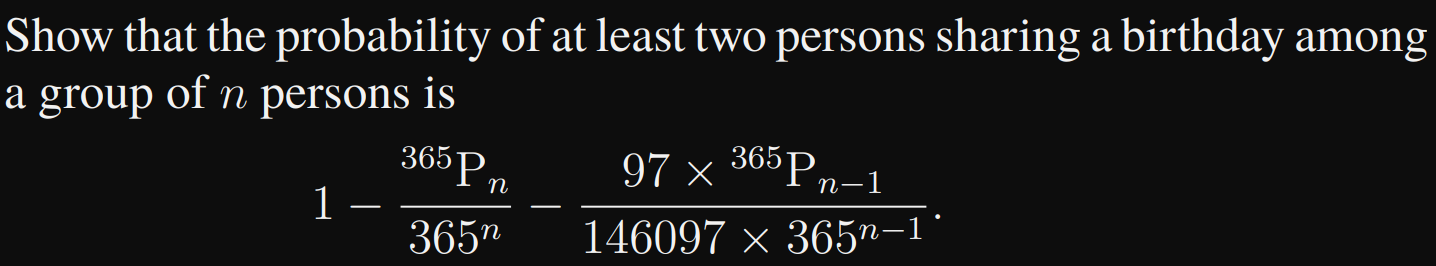
\includegraphics[scale=0.4]{ex01.png}
    \caption{Excercise Problem 01 from Course Notes}
    \label{fig:enter-label}
\end{figure}

\begin{proof}
\begin{center}
    
    At least 2 persons sharing a DOB
    $$=1- \text{(no person sharing a DOB)}$$
    $$= 1- \text{(no person born on 29th FEB} + \text{one person born on 29th FEB)}$$
    $$= 1 - \frac{365Pn}{365^n}$$

    Now for a 400 years leap year cycle\\
    leap year = $\frac{400}{4}$ - 4 + 1 = 100 - 3 =97\\
    total days in a cycle = $400 \times 365 + 97$ = 146097\\
    $\therefore$
    $$= 1 - \frac{\perm{365}{n}}{365^n} - \frac{97}{146097}\times \frac{\perm{365}{n-1}}{365^{n-1}}$$

    
\end{center}
\end{proof}


\section{Special Class/Talk on Paradoxes in Probability By Gaurav Banerjee (21MS) \\ 11th January 2024}
\subsection{Trivial Results:}
\subsubsection{Axioms of Probability:}
Let that set of outcomes be $\Omega$. $P(\Omega)$ be the total probability.
$\dots$ The same stuff from the class.

Collection of events are basically a set, whose elements can be assigned a probability.
Let the experiment be $\Psi$. $\cup_{i=1}^{\infty} A_i = E$ 
$P: E \to [0,1]$
\begin{enumerate}
    \item $P(\Omega) = 1$
    \item $P(\cup_{i=1}^{n} A_i)  = \sum_{i=1}^{n} P(A_i)$
\end{enumerate}
\begin{mdframed}
    Pain also gives you pleasure!!!
    $\dots$ if you take Maths Major.
\end{mdframed}
\subsubsection{Paradox 01:}
Probability of getting 2 consecutive heads in infinite tosses is 1, same for 2 consecutive head/tails is 1. Then the probability of n consecutive tosses is also 1.  Now, the probability of getting $\infty$ consecutive heads tends to 0. How?
Probability of getting k consecutive heads in infinite tosses be $P(A_k)$
Case 1:
first T then 

$P(A_k) = \frac{1}{2} P(a_k) + \frac{1}{2}^{k} + \sum_{i=2}^{k} P(T_1) P(A_k)$


$P(A_k) = \frac{1}{2} (P(A_k)) + \frac{1}{2}^k + \frac{1}{2}$


\subsubsection{Paradox 02 ( Bertrand Paradox):}

$A_1 \subset A_2 \dots $
$0< P(A_1) < P(A_2) < \dots <=1$
$\lim_{n \to \infty}P(\cup_{i=1}^{n} A_i) = $
$B_1 = A_1$
$B_2 = \frac{A_1}{A_2}$
$B_k = \frac{A_k}{\cup_{i=1}^{k-1} A_i}$
$\cup_{i=1}^{n} A_i B_i = \cup_{i=1}^{n} A_i$
$\cup_{i=1}^{\infty} A_i = \cup_{i=1}^{infty} B_i = A$
$\therefore \lim_{n \to \infty}P(\cup_{i=1}^{n} A_i) = $\lim_{n \to \infty}P(\cup_{i=1}^{n} B_i) = $\sum_{n \to \infty}P(\cup_{i=1}^{n} B_i) = $  
$\therefore \lim_{n \to \infty} P(a_n) = P(\lim_{n \to \infty} \cup_{i=1}^{n} B_i =P(\lim_{n \to \infty} \cup_{i=1}^{n} A_i  $



\subsection{Dirac Measure of Probability}

\section{Tutorial 02: 15th January 2024}
\subsection{Solving Exercises: }
\subsubsection{Problem 02:}
\begin{figure}[h]
    \centering
    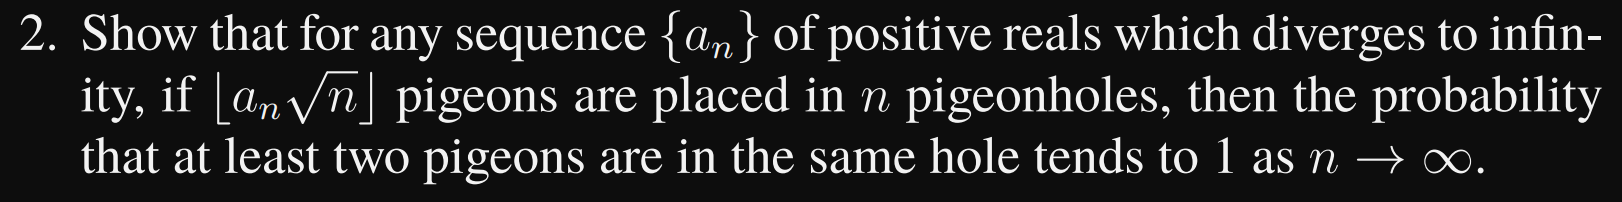
\includegraphics[scale = 0.3]{ex02.png}
    \caption{Problem 02 from Course Notes}
    \label{fig:enter-label}
\end{figure}
\subsubsection{Solution 02:}
\begin{proof}
    Tougher to show but can be done: $$1- \frac{\perm{n}{a_n \cdot \sqrt{n}}}{n^{a_n \cdot {\sqrt{n}}}} \quad \to 1 \quad if {a_n} \to \infty \quad n \floor{a_n\sqrt{n}}{}$$
   
\end{proof}


\section{Class Session : \\ 16th January 2024}
\subsection{Bonferroni's Inequality:}
\textbf{ Statement:} Probability space A_1, \dots, A_n are events in $\epsilon$, so\\
\[
P(A_1 \cap A_2 \cap \dots \cap A_n) \geq P(A_!) + \dots + P(A_n) - (n-1)
\]
\begin{proof}
    If for n=1, 
    \[
    P(a_1) \geq P(a_1) -0
    \]
    for n=2,\\
    \[
    P(a_1 \cup a_2) = P(A_1) + P(A_2) - P(A_1 \cap A_2)
    
    \]
    \[
    P(a_1 \cap a_2) = P(A_1) + P(A_2) - P(A_1 \cup A_2)
    \]
    \[
    P(a_1 \cup a_2) \leq 1 (\text{ Since } \epsilon: \to [0, \pi]
    \]
    \[
    \implies - (P(A_1 \cup A_2) \geq -1
    \]
    \[
    \implies P(a_1 \cap a_2) \geq P(A_1) + P(A_2) -1
    \]
    Induction hypothesis: The claim for $m \in \mathbb{N}$
    P(a_1 \cap a__m \cap A_{m+1}) \geq P(a) + P(b) -1
    = P(a_1 \cap a__m) + p(A_{m+1}) -1
    \geq P(A_1) + \dots + P(A_m) - (m-1) + P(A_{m+1} +1
    = P(A_1) + \dots + P(A_m) + P(A_{m+1} -m
\end{proof}

\subsection{Bayseian Probability:}
$(\Omega, \epsilon, P)$ : = Probability Space, then $B \in \epsilon$ has already occurred has the result of an random experiment. $A\in \epsilon$, if $A \cap B = \phi$, then A hasn't occurred. If $A \cap B \neq \phi$, then the probability of this event is measured in relation to the random experiment of B.

\subsection{Conditional Probability:}
Let $ B \in \epsilon $ be st $P(B) > 0$. Then for $A\in \epsilon$, we define $P(A|B) = \frac{P(A \cap B)}{P(B)}$.
\\
Imparticular, $P(B|B) = 1$ [compare it to $P(\Omega) =1$]


\subsubsection{Lemma of Total Probability:}
Let $(\Omega, \epsilonP$ be our probability space and let ${A}_{i=o}^{\infty}$ be pairwise mutually exclusive events st P(A_o) = 0 and 
P(A_i) >0 $\forall i \in \mathbb{N}$. Then for any $B\in \epsilon$, we have $P(B) = \sum_{i=1}^{\infty} P(A_i) P(B|A_i)$



%Trivial total prob fig

If $A_1 \cup \dots \cup A_n = \Omega$
$P(B) = P(B\cap A_o) + P(B\cap A_1) + \dots P(B\cap A_n)$ 
$\since P(B\cap A_o) =0$
$P(B\cap A_1 ) + \dots + P(B \cap A_n)$
\[
= \sum_{i=1}^{n} P(A_i) P(B|A_i)
\]
\textbf{Notes:}
\[
P(B|A_i) = \frac{ P(B \cap A_i)}{A_i}
\]
\[
\implies P(A_I)P(B|A_i) = P(B \cap A_i)
\]

\subsection{Bayes' Theorem:}
Let $(\Omega, \epsilon, P)$ be the probability Space and let ${A_i}_{i=1}^{\infty}$ be pair-wise mutually exclusive and exhaustive events with $P(A_i)>0 $   $\forall i \in \mathbb N$. Then for any $B \in \epsilon$, with P(B)>0, we have 
\[
P(A_j|B) = \frac{P(A_j)P(B|A_j)}{\sum_{i=1}^{\infty}P(A_i)P(B|A_i)}
\]
\begin{proof}
    \[
    P(A_j|B) = \frac{P(A_j \cap \B)}{P(B) = \frac{P(A_j)P(B|A_j)}{\sum_{i=1}^{\infty}P(A_i)P(B|A_i)}}
    \]
\end{proof}
\subsubsection{Example 01:}
Let's roll a fair die till we get an outcome of 6. Call $A_n$ the event in which we stop at the nth roll. Let B be the event that all the outcomes preceding the last one are odd. Determine $P(A_m|B)$
\begin{proof}
\[
P(A_m) = \frac{1}{6} \cdot \frac{5}{6}^{n-1}
    P(B|A_m) = \frac{P(B \cap A_m}{P(A_m} = \frac{\frac{1}{6} \cdot \frac{3}{6}^{n-1}}{\frac{1}{6} \cdot \frac{5}{6}^{n-1}}
    = \frac{3}{5}^{n-1}
\]
    
    $P(A_m|B)$ = \frac{P(A_m)P(B|A_m)}{\sum_{m=1}^{\infty}P(A_m)P(B|A_m)} = \frac{\frac{1}{6}\frac{5}{6}^{n-1}\frac{3}{6}^{m-1}}{\sum_{n=1}^{\infty}\frac{1}{6}\frac{5}{6}^{n-1}}\frac{3}{6}^{n-1} = \frac{\frac{1}{2^{n-1}}}{\sum_{n=1}^{\infty}\frac{1}{2^{n-1}}} =\frac{1}{2^m}
\end{proof}
\subsubsection{Example 02:}

Suppose you find someone interesting and you'd like to ask him/her out for coffee. Let's assume there are three mutually exclusive, exhaustive and equally likely cases:
\begin{enumerate}[label=(\Alph*)]
    \item He/she finds you interesting as well
    \item He/she feels indifferent towards you
    \item He/she is repulsed by you
\end{enumerate}

\printindex
\[
P(Y|A) = 0.9
\]
\[
P(Y|B) = 0.5
\]
\[
P(Y|C) = 0.1
\]
\begin{enumerate}[label=(\roman*)]
    \item Find the probability that He/she accepts your invitation
    \item Given that he/she accepts your invitation, find the probability that he/she finds you interesting as well.
    
\end{enumerate}
\begin{proof}
    \[
    P(Y) = P(Y|A)P(A) + P(Y|B)P(B) + P(Y|B)P(B)
    \]
\[
\since Mutually Exclusive and exhaustive(P(A \cup B \cup C) =1)
P(A) = P(B) = P(C) = \frac{1}{3}
\]

  \[
    P(Y) = \frac{1}{3}(P(Y|A) + P(Y|B) + P(Y|B)) = 0.5
    \]
Now, for the second part,
\[
P(A|Y) = \frac{P(Y|A) \cdot P(A)}{P(Y)} = \frac{0.9 \times \frac{1}{3}}{0.5} = 0.6
\]
    
\end{proof}
\subsubsection{Example 03:}
One of your friends knows that among the three shown boxes, there lies a coin in one, so now she lifts the box to show the box w/o the coin, how the probability changes when nothing being there is revealed?
\textbf{Solution:}
A: Your initial Guess to be right 
$A^c$ : your initial guess is wrong
L: your friend lifts an empty box
We must compare, $P(A|L)$ and $(P(A^c|L))$,
\[
P(L) = P(L|A) =1 \text{ [Since both are the same events]}
\]
\[
P(A|L) = \frac{P(A) \cdot P(L|A)}{P(L)} = \frac{\frac{1}{3}}{1}
\]
\[
P(A^c|L) =1 - P(A|L) = \frac{2}{3}

\]

\begin{tabular}{||p {3 cm}|p{1cm}|p{1 cm}|p{1 cm}| p {1 cm}||}
    \hline
    & Initial Guess & Coin is under & Stick to initial guess & Switch \\
    \hline
    \hline
    1 & A & A & ok & x \\
    2 & C & A & x & ok \\
    3 & A & A & ok & x \\
    4 & A & B & x & ok \\
    5 & B & B & ok & x \\
    6 & C & B & x & ok \\
    7 & A & C & x & ok \\
    8 & B & C & x & ok \\
    9 & C & C & ok & x \\
    \hline
\end{tabular}


\begin{mdframed}[style = HW]
    Random Monty-Hall. Your friend does not know where the coin hides and she lifts a cup which happens to be empty (by chance). Would you still switch?
\end{mdframed}
 \subsection{Probabilistic Notion of Independence:}
 Let A, B $\in \epsilon$ be two events such that the occurrence of any of them does not influence the other, in other words, $P{A|B) = P(A) \text{,and }P(B|A) = P(B)$
\[
\impliedby P{A|B) = \frac{P(A \cap B )}{P(B)} = P(A) \dots
\]
\[
P(A \cap B ) = P(A) \cdot P(B)
\]
[could be taken as the formal definition of independence]

\subsection{Mutual v/s Pair-wise Independent}

If $S \subseteq \epsilon$ st $P(A \cap B ) = P(A) P(B), \forall A,B \in S$, we say the events in S are pairwise independent, whereas if $\forall T \in S$, we have $P(\bigcap_{A \in T} A) = \prod_{A \in T} P(A)$, the events in S are called mutually independent.

\subsubsection{Example:}
Suppose we roll a fair tetrahedral die and let 
\begin{enumerate}
    \item A: = 
\end{enumerate}


\section{Class Session 07 \\ 18th January 2024}
\subsection{Back On Statistician joke:}

The statistician computed the probability of having a bomb $B_1$ on the plane. Let's say $P(B_1) = p$. Apparently, wonder the assumption of independence, he computed the probability of having two bombs on the plane.
\[
P(B_1 \cap B_2) = P(B_1)\cdot P(B_2) = p^2
\]
Instead, he should have calculated 
\[
P(B_2| B_1) = \frac{ P(B_1 \cap B_2) }{P(B_1)} = \frac{p^2}{p} = p 
\]

\subsection{Open Conjecture: Erdoss (1976):}
Given $m \in \mathbb N$ , $m \geq 3$, any sequence with $\alpha_n \in \mathbb N$ such that $\sum_{n+1}^{\infty } \alpha_n = \infty$, we have an arithmatic progression of length m in {${\alpha_n}$}.\\

2,3,5,7,11,...
$\sum_{p < n}^{\infty } \frac{1}{p} \dots$ diverges\\
{$\{3,5,7\}$} Arithmetic Progression of length 3\\
{${5,11,17,23,29} $} Arithmetic Progression of length 5\\
{${7, 37, 67, 97, 127, 157}$} Arithmetic Progression of length 6\\

\subsection{Green -Tao, (2004)}
The Erdos conjecture holds for prime numbers.
\subsection{Bloom- Sisask, (2020)}
The Erdos conjecture holds true for m=3 case.


\subsection{}


\section{Class Session 07: 22nd January 2024}
\subsection{Random Monty Hall:}

A: Your initial guess is correct.\\
L: Your friend picks a cup which happens to be empty.\\
We must compare $P(A|L)$ and $P(A^c|L)$, then 
$P(L|A)=1$
$$P(L|A^c)= \frac{1}{2}$$
$$then, P(A|L)= \frac{P(A \cap L)}{P(L)} = \frac{P(A) \cdot P(L|A)}{P(A)P(L|A) + P(A^c)P(L|A^c)}$$
$$= \frac{\frac{1}{3} \times 1}{\frac{1}{3} \times 1 + \frac{2}{3} \times \frac{1}{2}}$$
$$= \frac{1}{2}$$
\begin{quote}
Next, the assignment problem will have K cups. This guy is making us insane in the world of probabilities probably.
    
\end{quote}

$\implies$ There's no adventure in switching!!!

\subsection{Base Rate Fallacy/ False Positive Paradox:}
Consider a very rare disease, which affects 0.1 \% of the population and let there be a test for this disease with $99\%$ sensitivity (The TRUE Positive) and 99\% specificity (True Negative). Sensitivity  is the 100\% probability
\begin{enumerate}[label= Roman]
    \item Sensitivity is the 100\times probability of identification of the disease in a person when he/she is affectedd by that disease.
    \item Specificity of a test is 100\times the probability of correctly identifying a case.
\end{enumerate}

$\therefore \frac{\text{Sensitivity}}{100} = P(P|D) = 0.99$
$$\therefore \frac{\text{Specificity}}{100} = P(N|D^c) = 0.99$$
$$P(D) = 0.001$$
Here,
$D\implies$ Presence of The Disease\\
$P: \implies$ Positive test Result
$N: \implies $ Negative 
\textbf{Question:} 
\begin{enumerate}
    \item Find the probability that a person has the disease if he/she tests positive [(P(D|P)]
    \item Given that a person has tested positive once, find the probability that he/she has the disease if he/she tests positive again.
     \item Given that a person has tested positive twice, find the probability that he/she has the disease if he/she tests positive again.
\end{enumerate}
\textbf{Answers:}
\begin{enumerate}
    \item $\implies 0.09$
    \item $\implies 0.91$
    \item $\implies 0.999$
\end{enumerate}


\section{Class Session 09: \\23rd January 2024}
\subsection{Random Variables:}
\subsubsection{Roll A die:}
You'll get an outcome in ${1,2,3,4,5,6}$

\subsubsection{You Ask for a Girl's Number:}
You will get a 10-digit no.s (Assuming you'll get a response in numbers and not physical action)

\subsubsection{Guess The First Letter of a person's Name:}
\subsubsection{Guess The Favourite color of a person:}
\subsection{Quantifying These Stuff:}
We may quantify these by assigning 26 variables to the Alphabet.
$\exists$ Analogy between measurable and continuous functions.
\\
\textbf{Definition: } Let $f: S \to \prime S$ be continuous $\impliedby$ For every open set $\bigoplus ' \subseteq S'$, then  $f^{-1} (\bigoplus ') \subseteq S$ is open.
Let $f: S \to  S' (\text{Measurable spaces})$ [This means pre-image of the measurable subset of $S'$ is a measurable subset of S] be a measurable function, then,
\[
\Omega \to \mathbb{R} \dots \text{Probability/events to length/intervals}
\]

If $\bigoplus ' \subseteq S'$ is measurable then $f^{-1} (\bigoplus ') \subseteq S$ is also measurable. 

\subsection{Definition of a Random Variable:}

This is a real-valued function on the sample space st the pre-image of every interval is an event.
By \textbf{Random Variable (for this course)} we'll always mean a real-valued  Random Variable.
\subsection{Definition : Probability Distribution of a Number:}

Let $(\Omega,\epsilon, P)$ be a probability space and $X: \Omega \to \mathbb{R}$ be a random variable, then $X$ translates $(\Omega,\epsilon, P)$ to $(\mathbb{R},\epsilon_X, P_X)$, where 
\[
\epsilon_X = \{A \subseteq \mathbb{R}| X^{-1}(A) \in \epsilon\}
\]
\[
P_X = P(X^{-1}(A))
\]
\subsubsection{Non-measurable Subsets of $\mathbb{R}$}

\textbf{Vitali-sets:} $[0,1]  \backslash  \mathbb{Q} = \mathbb{Q}' $ , these are non-measurable.
Then $\forall q_i \in [-1,1] \cap \mathbb{Q}$, we have $q_i + \mathbb{Q}$.
Enumerate the rationals in $[-1,1]$, as $\{q_1,q_2, \dots\}$, then consider {$q_i + \mathbb{Q}'$}, we have \\$q_i + \mathbb{Q}' \subseteq [1,-2]$, 
\[
l(q_i + \mathbb{Q}') = l(\mathbb{Q})= c
\]
\[
c \leq \sum_{i=1}^{\infty} l(q_i + \mathbb{Q}') \leq 3
\]
\subsubsection{Notations:}
Henceforth, we'll use the notations $P_X(A)$ and P($X \in A$) interchangeably . In particular, we'll write $P_X([-\infty, a])$ as $P(X \leq a)$

\subsection{Redefining the Random Variable:}

\[
X : \Omega \to \mathbb{R}
\]
such that, \[
X^{-1} ((- \infty, a] \in \epsilon) \forall a \in \mathbb{R}
\]
\subsubsection{Example:}
\[
(- \infty, a] = \cup_{n=1}^{\infty} (- \infty, a - \frac{1}{n})
\]
\[
(a,b) \implies \mathbb{R} \backslash ((-\infty, a] \cup [b,\infty)) = \mathbb{R} \backslash ((-\infty, a] \cup (-\infty,b)^c)
\]
\subsubsection{Lemma:}

\[
\forall x \in \mathbb{R}\text{, we have} \{x\} \in \epsilon_X.
\]
\begin{proof}
    \[
    \{x\} = [x,x] = ((-\infty, x)\text{$\in \epsilon_X$} \cup (x,\infty)\text{$\in \epsilon_X$})^c
    \]
    $\epsilon_X $ is closed under countable unions and complementation. So, ${x} \in \epsilon_x$
    
\end{proof}

\subsubsection{Corollary:}
\[
\forall r.v X
\]




\end{document}





